\chapter{Asking Millionaires How They Got Rich (Miami)}

These notes follow the Miami sequence in the School of Hard Knocks interview series and are curated by LazyingArt LLC. The lecture is built less like a formal theorem-proof development than like a guided tour through a set of local scaling problems: how a business escapes the solopreneur bottleneck, how branding separates price from cost, how a firm crosses from seven figures to nine, how data begins to govern growth, how capital should or should not be stored, and what survives a recession. Our task is to keep the lecture's order of discovery intact while imposing just enough notation to prevent unlike quantities from being confused with one another.

\section{Opening Measure of Wealth}

The lecture opens by showing us outcomes before it explains them. We hear about a business that did \(149\,\mathrm{M}\) last year and may do roughly double, a best year of \(10\,\mathrm{M}\), a surgeon's \(1.5\,\mathrm{M}\), and the millionaire-to-billionaire trajectory that will culminate in the Grant Cardone interview. Only after this montage does the host reset the scene: Miami is a city with a high density of millionaires, and the point of the exercise is to ask not merely what people made, but how they became successful and what a younger viewer can learn from the path.

The first discipline of the chapter is therefore classification. The lecture repeatedly asks for ``the most amount of money,'' but the answer may refer to company revenue, gross receipts, net receipts, assets under management, or personal income. We keep those objects separate from the start.

\begin{table}[h]
\centering
\begin{tabular}{llll}
\hline
Case & Quantity & Object & Type \\
\hline
Solar CEO & \(149\,\mathrm{M}\) & prior-year business volume & revenue \\
Solar CEO & \(\approx 300\,\mathrm{M}\) & projected business volume & revenue \\
First operator & \(5.0\,\mathrm{M}\) & largest month gross & gross business amount \\
First operator & \(3.9\,\mathrm{M}\) & largest month net & net business amount \\
Robert Miller & \(50\,\mathrm{M}\) & year-end target & assets under management \\
Brandon Carter & \(10\,\mathrm{M}\) & best year, with businesses and investments & composite annual amount \\
Cardiovascular surgeon & \(1.5\,\mathrm{M}\) & best year & personal income \\
\hline
\end{tabular}
\caption{Transcript-derived quantities. The same interview prompt refers to different financial objects in different cases.}
\end{table}

Throughout the chapter we write \(R\) for top-line revenue, \(G\) for gross, \(N\) for net, \(L\) for lead flow, \(D\) for documentation or SOP coverage, and \(H\) for time horizon. With those symbols in place, the lecture becomes much sharper: we are not looking at a bag of success stories, but at a series of attempts to identify the operator that maps one sort of input into one sort of financial result.

\section{First Operator: Scale Through Delegation, Sales, and Time Horizon}

The first full case follows the lecture's characteristic sequence. The host asks what industry the speaker pursued, then asks for the biggest amount of money made in a single year, and only then asks for the mechanism. The answer begins with e-commerce and moves into mergers and acquisitions and real estate. The first secure numerical anchor is a largest month with
\begin{align}
G_m &= 5.0\,\mathrm{M}, &
N_m &= 3.9\,\mathrm{M}.
\end{align}
The speaker adds that the current year is already ahead of the previous one. A later line about ``\(10\,\mathrm{M}\) gross'' and ``\(7.9\) net'' is transcriptually unstable, so we do not build any exact algebra on it.

\paragraph{Claim.}
The speaker attributes the year's improvement not to a sudden flash of genius but to a structural change: the building of a team and a system. The lecture is careful here. It does not merely praise delegation in the abstract. It puts delegation in causal position. The solopreneur who insists on doing everything personally has a business whose scale is bounded by one person's bandwidth.

\paragraph{Mechanism.}
The argument can be compressed into the transcript-derived chain
\begin{equation}
\text{delegation}+\text{team}+\text{system}
\rightarrow
\text{capacity}
\rightarrow
\text{growth}.
\end{equation}
This is not a theorem. It is the lecture's first operating rule.

\paragraph{Worked calculation.}
The transcript gives us one clean piece of arithmetic, namely the relation between the cited monthly gross and net amounts. We compute
\begin{align}
m_{\text{net}}
=
\frac{N_m}{G_m}
=
\frac{3.9}{5.0}
\approx 0.78.
\end{align}
So the spoken month corresponds to an implied net-to-gross fraction of roughly \(78\%\). The point of the exercise is not to universalize that ratio, but to show how even a highly conversational lecture carries numerical structure if we pause to extract it.

The speaker then moves from organizational structure to sales. ``Sales is psychology'' is the governing slogan, and the lecture illustrates the slogan with a luxury-store anecdote: low-cost shoes are relabeled and repriced as luxury goods, and buyers willingly pay the luxury tag. The sequence matters. First we saw that a business can stall because it is organized badly. Now we are shown that a business can sell at high volume because price is mediated by perception, scarcity, and branding.

\subsection{Question \& Answer}

\paragraph{Question.}
Why do solopreneurs stall, and why do branded goods sell so far above their apparent intrinsic cost?

\paragraph{Answer.}
The lecture gives one organizational answer and one market answer, but the two are structurally parallel. A solopreneur stalls because too many functions are concentrated in one person. A branded product commands a premium because too much value is concentrated in one perception. In the first case, the scarce resource is the founder's finite attention. In the second, the scarce resource is the buyer's sense of status, exclusivity, and access.

The arithmetic shadow of the branding example is easy to write down. If the shoes cost about \(20\) dollars and are tagged in the range \(800\) to \(900\), then
\begin{align}
c_{\text{shoe}} &= 20, &
p_{\text{tag}} &\in [800,900], &
\frac{p_{\text{tag}}}{c_{\text{shoe}}} &\in [40,45].
\end{align}
A price multiple of roughly \(40\) to \(45\) is the numerical residue of the claim that branding can stretch willingness to pay far beyond cost.

The lecture then swings once more, now from pricing psychology to financial advice for younger people. The speaker warns against social-media optics, conspicuous consumption, and living for the short horizon. We are told to live below our means, invest, accumulate, and let compounding do the slow work. The transcript gives no exact formula, but the canonical reconstruction is straightforward: if one contributes a fixed amount \(a\) each year at rate \(r\) for \(n\) years, then
\begin{equation}
FV_n = a\,\frac{(1+r)^n-1}{r}.
\end{equation}
This formula is not quoted by the speaker; it is our careful completion of the compounding doctrine.

What the lecture insists on, however, is less the formula than the horizon:
\begin{equation}
H_{\text{short}}\in\{\text{weeks},\text{months}\},
\qquad
H_{\text{long}}\in\{\text{years},\text{decades}\}.
\end{equation}
The difference between apparent wealth and durable wealth is presented as a difference in time scale. Poor people, we are told, think in weeks and months; rich people think in years and decades. The line ``this is 100 years'' is too uncertain to treat literally, but the long-horizon point is unmistakable.

\section{Solar Scale: From Craft Knowledge to Nine-Figure Systems}

At this point the host recaps the previous interview, praises what was learned, and then raises the stakes: we move to Sunny Isles to meet a nine-figure solar-company CEO. The rhythm is deliberate. One case gives us a rule; the next case tests whether that rule survives at a much larger scale.

The solar CEO begins not with systems talk but with craft. He went door to door, learned the product, learned the customer base, learned the proposal, moved into installation, learned the technology, and assembled teams of construction workers, engineers, and designers. This narrated path through the stack is important. It gives the later scaling claims a concrete base. The speaker is not describing a company from above; he is describing the route by which he entered the moving parts of the company.

The lecture then gives a compressed law of compensation:
\begin{equation}
\text{Pay} \propto \text{problem size solved}.
\end{equation}
That line is attributed via Elon Musk, but it does real work in the chapter. It tells us how to read the move from small business to large enterprise: compensation scales with the magnitude of the operational problem one can address.

The numerical part is clean. The business did \(149\,\mathrm{M}\) last year, and the claim is that it should do double this year. So the host rounds out the implied update:
\begin{align}
R_{\text{solar},y+1}
&\approx 2R_{\text{solar},y}
=2(149\,\mathrm{M}) \\
&= 298\,\mathrm{M}
\approx 300\,\mathrm{M}.
\end{align}

The next question is the lecture's central scaling question: what takes a firm from seven figures to eight and then from eight to nine? The answer is staged explicitly enough that it can be preserved as a simple diagram.

\begin{figure}[h]
\centering
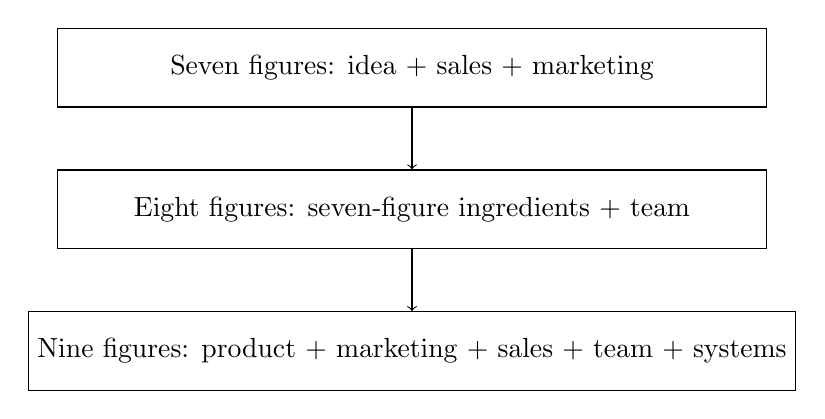
\begin{tikzpicture}[x=1cm,y=1cm]
\node[draw, minimum width=9cm, minimum height=1cm] (s7) at (0,0) {Seven figures: idea \(+\) sales \(+\) marketing};
\node[draw, minimum width=9cm, minimum height=1cm] (s8) at (0,-1.8) {Eight figures: seven-figure ingredients \(+\) team};
\node[draw, minimum width=9cm, minimum height=1cm] (s9) at (0,-3.6) {Nine figures: product \(+\) marketing \(+\) sales \(+\) team \(+\) systems};
\draw[->] (s7) -- (s8);
\draw[->] (s8) -- (s9);
\end{tikzpicture}
\caption{A transcript-derived scaling ladder. The lecture presents the nine-figure transition not as ``more hustle'' but as the arrival of systems.}
\end{figure}

In compact notation:
\begin{align}
\mathcal{D}_7 &= \{\text{idea},\text{sales},\text{marketing}\},\\
\mathcal{D}_8 &= \mathcal{D}_7\cup\{\text{team}\},\\
\mathcal{D}_9 &= \{\text{product},\text{marketing},\text{sales},\text{team},\text{systems}\}.
\end{align}
The lecture's key move is that the last step is not merely additive. The object itself changes. A nine-figure business must cease to be a founder's extended arm and become something more machine-like.

\subsection{Question \& Answer}

\paragraph{Question.}
What actually takes a firm from eight figures to nine?

\paragraph{Answer.}
The lecture's answer is not charisma, not raw effort, and not even team quality by itself. It is documented systems, that is, SOPs that make recurring functions transferable. The speaker exaggerates for emphasis by saying that there is an SOP even for going to the bathroom or making coffee. The exaggeration sharpens the point: the decisive object is repeatability, not brilliance.

If we let \(D\) denote documentation coverage over recurring business functions, then the argument is
\begin{equation}
D \uparrow
\quad \Longrightarrow \quad
\text{transferability} \uparrow
\quad \Longrightarrow \quad
\text{CEO dependence} \downarrow
\quad \Longrightarrow \quad
\text{system dependence} \uparrow.
\end{equation}
If the founder is sick and a colleague can still execute the function from documentation, then the organization has crossed a threshold. It is no longer relying primarily on the CEO; it is relying on the machine.

The lecture then pivots, while still inside the solar segment, from systems to capital deployment. ``Spend your money,'' the speaker says, not because accumulation is meaningless, but because idle money in a bank account is compared to a Bugatti with no gasoline. This is the first explicit collision in the lecture between store-of-value thinking and fuel-for-growth thinking, and it prepares the sharper version of that collision in the Grant Cardone finale.

\section{Data, Environment, and Revenue Attachment}

The host next moves us back to Brickell and introduces Robert Miller. The transition is handled in the lecture through environment: Miami is not presented simply as an expensive lifestyle choice, but as a denser entrepreneurial field, a home base, a network, a beach, and a financial district. That is, environment enters the lecture as an input into ambition and execution rather than as a decorative backdrop.

Only after that environmental frame do we get the business profile: several businesses, early exposure to digital currencies, digital marketing, e-commerce, crypto, about \(15\,\mathrm{M}\) this year, \(20\) to \(25\,\mathrm{M}\) projected next year, and a target of \(50\,\mathrm{M}\) in assets under management. The host then asks the right question: what actually pushed the business from seven figures to eight?

The answer is delivered in a phrase that sounds almost too simple: ``follow the graph.'' The lecture immediately knows that this phrase is not yet intelligible and pauses to unpack it.

\subsection{Question \& Answer}

\paragraph{Question.}
What does it mean to ``follow the graph''?

\paragraph{Answer.}
The first graph is the revenue graph, understood as a spoken summary of how sales and marketing are performing. The second is the social-media side: impressions, content, algorithmic movement. The point is not to worship a graph as an image. The point is to force the entrepreneur into contact with measurable feedback.

The first causal chain is
\begin{equation}
\text{Marketing} \rightarrow L \rightarrow \text{Sales} \rightarrow R,
\end{equation}
where \(L\) is lead flow and \(R\) is revenue. This chain matters because the speaker's financial advice is to attach oneself to revenue. The closer one moves upstream to lead generation, the more central one becomes to the firm's actual money-making process.

The second chain is the decision chain:
\begin{equation}
\text{Data} \rightarrow \text{better decisions} \rightarrow \text{better improvements} \rightarrow \text{growth}.
\end{equation}
The lecture warns that entrepreneurs often psych themselves out by refusing to look at data. In that sense, ``follow the graph'' means: do not substitute mood for measurement.

We may summarize the segment this way. Early growth can be hustled into existence. Later growth requires instruments. The speaker's image of ``parabolic growth'' should be read rhetorically, but the underlying operational point is clear: once the business has enough data to guide decisions, improvements can become more targeted and compounding in effect rather than merely strenuous.

\section{Durability, Excellence, and the Long Game}

At this stage the host pauses to reflect on what it feels like to spend time around eight- and nine-figure operators. This short bridge is worth keeping, because it performs an important pedagogical function: it converts the previous interviews from isolated facts into a single atmosphere. The effect of the atmosphere, the host says, is not complacency but the feeling that current achievement is still far below the top of the mountain.

The lecture then widens again. Brandon Carter is introduced as a fitness entrepreneur who made more than \(10\,\mathrm{M}\) in a year, but the operative content of his interview is not the number. It is the rule for bad times: sweat during peace, bleed less during war. The recession question follows naturally. What makes a business recession-proof, or at least recession-resistant?

A compact way of organizing the answer is
\begin{equation}
\mathcal{R}\sim \ell+\text{asset-backed access}+\sigma,
\end{equation}
where \(\ell\) is liquidity or immediate access to money, and \(\sigma\) is portable, monetizable skill, especially marketing and sales ability. This is only a mnemonic reconstruction of the interview's logic. The real content is qualitative: have money or access to it, have assets that can be borrowed against, and have a skill that can turn into cash if conditions deteriorate.

The surgeon's interview then changes the register in a useful way. Here the lecture moves away from entrepreneurial machinery and back toward professional vocation. The speaker's motivation is deeply personal, and the key rule is not to optimize for money directly. Excellence, service, and sacrificial focus come first; the money follows. This is a necessary counterweight in the chapter. Without it, the book would flatten every form of success into one entrepreneurial template, which the lecture itself does not do.

\section{Capital Velocity and the Puzzle of Going to Zero}

The final movement returns to the opening promise. The host tells us that Grant Cardone was one of the first entrepreneurs he watched when he first became serious about financial freedom and business. This matters, because the finale is not merely another interview; it is staged as a meeting with one of the formative figures behind the whole series' worldview.

Cardone's answer to the question about financial advice is intentionally provocative. He first says that money is just a tool. He then recounts the setup of \emph{Undercover Billionaire}: \(100\) dollars, \(90\) days, no name, and a target of \(10\,\mathrm{M}\). Instead of asking how to preserve the \(100\), he asks how to add zeros. His response is to go straight to zero.

\subsection{Question \& Answer}

\paragraph{Question.}
Why ``go to zero''? Why strip away the initial money rather than manage it carefully?

\paragraph{Answer.}
The point is strategic, not literal. ``Go to zero'' is a refusal to treat money-management as the entrepreneur's primary problem. Cardone's claim is that the relevant scarcity is not mainly cash but the ability to raise, deploy, and multiply capital through people, opportunity, brand, and action.

The rhetorical puzzle can be written as
\begin{equation}
100 \longrightarrow 0 \longrightarrow 10\,\mathrm{M},
\end{equation}
but this must not be mistaken for a numerical update rule. It is a doctrine of capital velocity. Idle money is treated as inert; deployed money is treated as productive:
\begin{equation}
K_{\text{idle}} \rightarrow 0,
\qquad
K_{\text{deploy}}
=
K_{\text{business}}
+
K_{\text{brand}}
+
K_{\text{knowledge}}
+
K_{\text{real assets}}.
\end{equation}

The internal logic proceeds in four steps:
\begin{enumerate}
\item Reframe the problem from preserving \(100\) dollars to adding zeros at speed.
\item Reject the tendency to ``manage money'' as the central entrepreneurial act.
\item Reinvest into business, marketing, brand, information, confidence, and speed.
\item When capital remains after that, move it into real assets, above all real estate.
\end{enumerate}

Here the lecture reaches its sharpest internal contradiction. Earlier we were told to live below our means, invest steadily, use compounding, and think in decades. Here we are told not to save money, not to plan for retirement, and to push every available dollar back into productive motion. The chapter is more faithful if it preserves this tension rather than resolving it prematurely. The lecture is not giving us one catechism. It is staging a live dispute about what money is for: protection, accumulation, multiplication, or motion.

The last claim is explicitly time-bound. Cardone says that the next \(18\) months will be the greatest real-estate opportunity of a lifetime, perhaps of the next \(50\) years. This is not a timeless axiom; it is a dated investment thesis attached to the lecture's moment.

\section{Summary}

The chapter begins with big numbers and spends the rest of its time trying to deserve them. The first operator teaches us that scale begins to change when delegation, team, and system replace the solopreneur fantasy. The pricing example teaches us that branding can separate price from cost by a large multiple. The compounding advice restores the long horizon. The solar CEO then refines the picture: seven figures, eight figures, and nine figures are not the same business with more volume, but different organizational forms, with SOPs marking the decisive passage to system dependence.

Robert Miller translates scale into measurement: follow the graph, follow the impressions, follow the content, and attach yourself to revenue. Brandon Carter broadens the lecture into resilience: liquidity, access to money, and portable skill matter when the cycle turns. The surgeon reminds us that excellence and service remain a separate route to durable income. Grant Cardone, finally, radicalizes the capital-allocation question by refusing to let idle cash sit still and by treating money as fuel rather than as a trophy.

If we keep the categories straight, the lecture stops being a blur of luxury, charisma, and headline claims. Revenue is not income; gross is not net; assets under management are not annual earnings; branding is not cost; data is not intuition; idle money is not deployed capital. Once those distinctions are made, the lecture unfolds as it intends to unfold: one interview at a time, one operator at a time, one local mechanism after another.